Nella sezione \emph{Utenti} è possibile visualizzare l'elenco di tutti gli utenti e cambiare la password corrispondente.

\begin{figure}[H]
    \begin{center}
    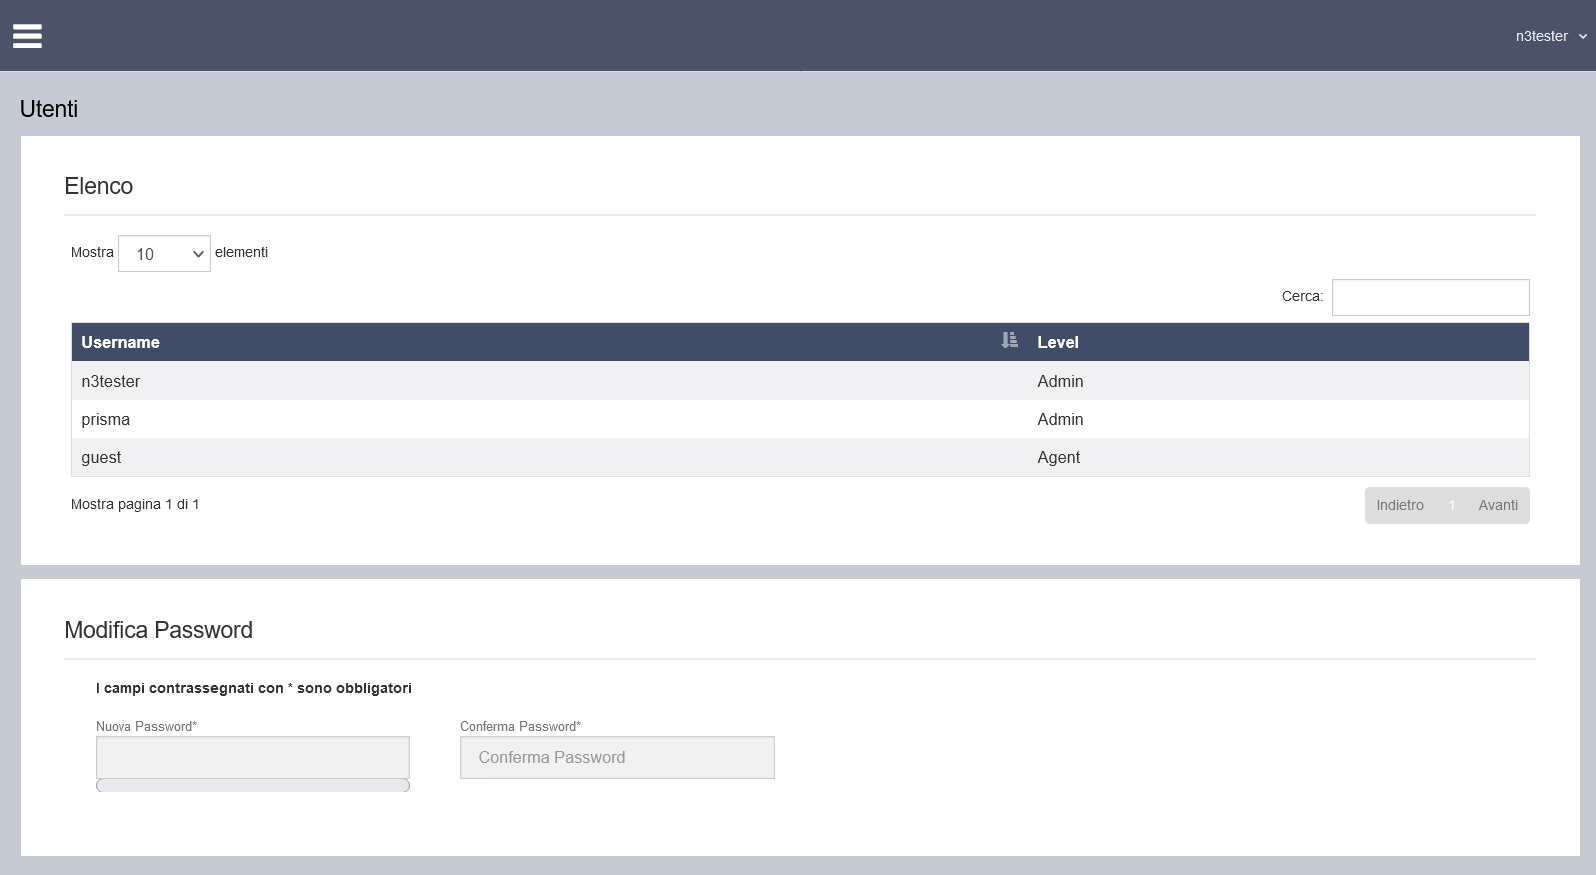
\includegraphics[width=\textwidth]{images/full-utenti.png}
        \caption{Sezione \emph{Utenti}.}
    \end{center}
\end{figure}

\subsection{Visualizzazione utenti}

La pagina mostra una tabella, implementata con DataTables, con l'elenco degli username di tutti gli utenti che possono accedere al sistema e il rispettivo livello (cfr. sezione \ref{sicurezza}).

\subsection{Cambio password}

\begin{wrapfigure}{l}{0.3\textwidth}
    \vspace{-4pt}
    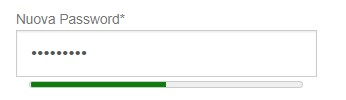
\includegraphics[width=0.3\textwidth]{images/pwd-strength-meter.jpg}
    \vspace{-24pt}
\end{wrapfigure}

Cliccando sulla relativa riga, si può accedere al cambio della password. Similmente ai campi nella configurazione automatica di Freeture (cfr. sezione \ref{ft-conf-automatica}), la password è gestita da un \textbf{sistema di validazione} e sottoposta ad un \textbf{controllo di robustezza} (\emph{strength meter}).

\subsection{Gestione sicurezza} \label{sicurezza}

Per rendere più sicura la web application dal momento che si interagisce con dati sensibili sul nodo, durante il lavoro è stato introdotto un sistema di sicurezza associato ai privilegi degli utenti. 

Come già accennato, ad ogni utente corrisponde un certo \textbf{livello}. I livelli possibili sono:
\begin{itemize}[noitemsep,nolistsep]
    \item \textbf{Admin}: livello amministratore, l'utente ha accesso a tutte le sezioni;
    \item \textbf{Agent}: livello base, l'utente ha accesso solo ad alcune sezioni non amministrative ma solo di consultazione.
\end{itemize}

Un utente \emph{Agent} condivide con gli amministratori solo la homepage e le  sezioni \emph{Calibrazioni}, \emph{Stack} e \emph{Detection}. Inoltre ha accesso alla sezione \emph{Configurazione FreeTure} (cfr. sezione \ref{sezione-freeture}) sebbene ridotta (cfr. figura \ref{fig:freeture-ridotto}), dove può solamente modificare l'anagrafica dell'\emph{observer} associato alla stazione.

Qualora un utente cerchi di accedere tramite URL a pagine non autorizzate, viene reindirizzato alla pagina di login.

\begin{figure}[H]
    \begin{center}
    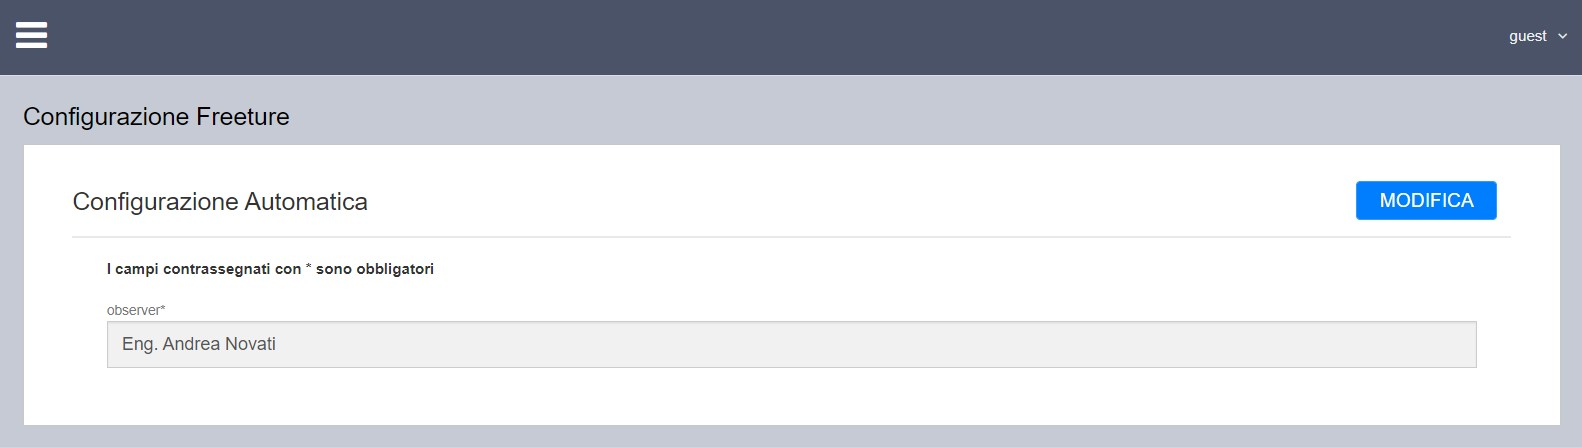
\includegraphics[width=\textwidth]{images/freeture-ridotto.jpg}
    \caption{Sezione \emph{Configurazione FreeTure} per gli utenti di livello \emph{Agent}.}
    \label{fig:freeture-ridotto}
    \end{center}
\end{figure}

\begin{figure}
    \begin{center}
    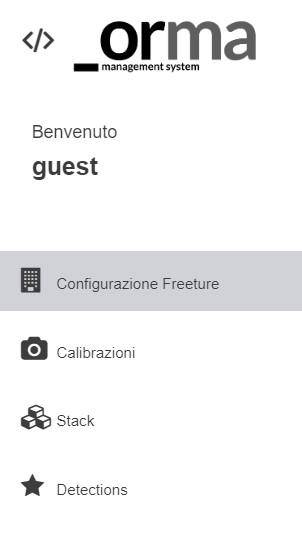
\includegraphics[width=0.4\textwidth]{images/menu-ridotto.jpg}
        \caption{Menu della web application per gli utenti di livello \emph{Agent}.}
        \label{fig:menu-ridotto}
    \end{center}
\end{figure}

